\chapter{Theory}
\section{What is a resonator?}
By resonator we mean a harmonic oscillator within which some quantity varies harmonically with time. In case of a helical resonator an alternating current in electrical circuit periodically transfers the inductive energy stored in a magnetic field of the helix into the capacitive electric field energy between the helix and the shield. When being stimulated by an RF signal with a natural frequency of the system, voltage amplitude grows until the damping mechanisms are strong enough to balance the resonant effect.

\section{Helical resonator models}
In order to create a helical resonator satisfying our experimental conditions and limitations we inevitably come to a need for a theoretical model that would be able to predict the essential characteristics of the resulting unit. The following sections aim to provide an overview and comparison between the models.

\subsection{Macalpine \& Schildknecht}
\begin{figure}[h!]
	\centering
	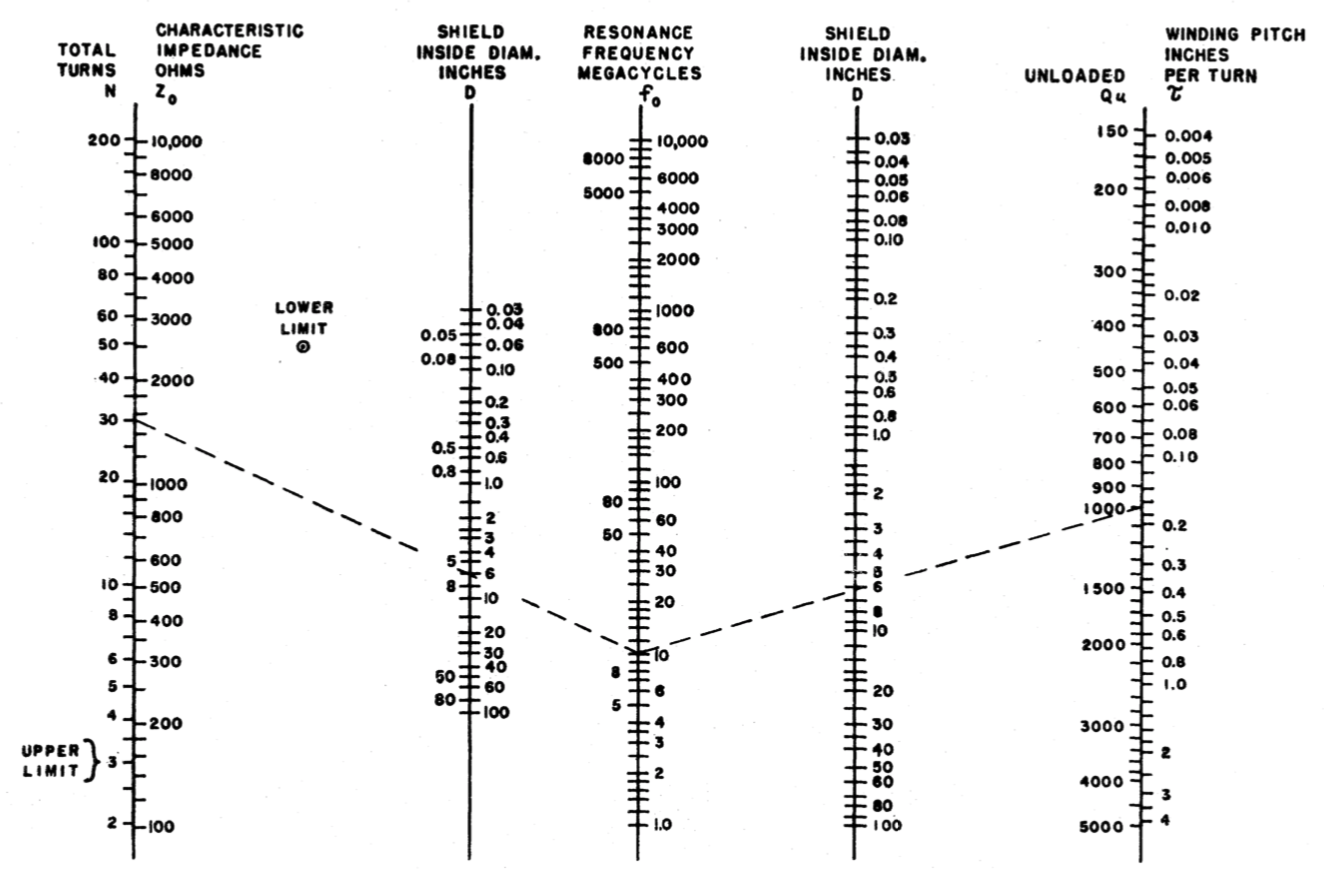
\includegraphics[width=.99\textwidth]{images/macalpine_chart}
	\caption{Design chart for quarter-wave helical resonators \cite{Macalpine2000}}
	\label{fig:macalpine_chart}
\end{figure}

A well-known approach \cite{Macalpine2000} for describing helical resonators was introduced in the same year as Richard Feynman's idea \cite{Feynman1960} to use quantum systems for computations. It was motivated by the possibility to reduce volume compared to TEM-mode coaxial-line resonators (90\% volume reduction for the reference case \cite{Macalpine2000}). While skipping a detailed theoretical analysis it nevertheless provides a basis for constructing a resonator: such as regions of usefulness, design considerations and a set of parameters' dependencies maximizing $Q$.

While describing essential properties of an unloaded helical quarter-wave resonator, this paper \cite{Macalpine2000} also predicts the shift of resonant frequency if an external load is connected. In order to define a new frequency one can make use of telegraph equations \cite{Rohde2009} by effectively treating the ion trap as a capacitor.

Important results of \cite{Macalpine2000} can be found in equations \ref{eq:macalpine} with parameters named as in the figure \ref{fig:helical_example}.
\begin{equation}
\begin{aligned}
	d/D &= 0.55\\
	b/d &= 1.5\\
	h &\approx (b + D/2)
\end{aligned}
\label{eq:macalpine}
\end{equation}
\subsection{Siverns et al.}
Unfortunately modeling an ion trap as a pure capacitive load is not always accurate. Introducing resistive losses imposes an additional shift of resonant frequency which pushes the deviation from self-resonant frequency even further. It is possible to tune the strength of the inductive coupling between the antenna and the main coil to compensate this shift while losing in efficiency.

These limitations of Macalpine's \& Schildknecht's \cite{Macalpine2000} model have been overcome in a newer paper \cite{Siverns2012} which takes the development of an amplifier, specifically for the needs of quantum computing, one step further. By taking a look at the joint resonator + ion trap system as a whole it aims to predict the effective $Q$ and frequency. This model ensures that it's possible to find optimal parameters for given experimental constraints.

While it is heavily recommended to check the original \cite{Siverns2012} paper to understand the theory behind calculations in appendix \ref{chapter:siverns_code} we will provide a short explanation of the exact usage below. All symbols correspond to \cite{Siverns2012}.

In our approach the only varying parameters are the diameter of a shield $D$ and the diameter of a helix $d$ with $\alpha = d / D$.

Formula for $Q$ from \cite{Siverns2012} depends on the inductance of the coil $L_C$ (\ref{eq:coil_inductance}), the real part of the total impedance $Z_{real}$ (\ref{eq:z_real}) and the target frequency $\omega_0$ ($2\pi * 40$ MHz). In the following equations we would expand dependencies until it is possible to express everything through our target and varying parameters.
\begin{equation}
	Q = \frac{L_C \; \omega_0}{Z_{real}}
	\label{eq:calc_q}
\end{equation}

Let's start with defining the inductance of the coil $L_C$. For a long solenoid as modified by the effect of the shield \cite{Macalpine2000} inductance can be described as linearly dependent on the length of the coil $b$ (\ref{eq:calc_b}) and a coefficient $K_{L_c}$ (\ref{eq:K_L_c}).
\begin{equation}
	L_C = b* K_{L_c}
	\label{eq:coil_inductance}
\end{equation}

The length of the coil $b$ can be derived \cite{Macalpine2000} from the height $h$ (56 mm) and the inner diameter $D$ of the shield. Since $D$ varies resulting $b$ might become less than 0 --- this case is handled properly in the appendix \ref{chapter:siverns_code}.
\begin{equation}
	b = h - D/2
	\label{eq:calc_b}
\end{equation}

The coefficient $K_{L_c}$ depends on the diameter of the helix $d$, the inner diameter $D$ of the shield and the winding pitch $\tau$ (\ref{eq:calc_tau}).
\begin{equation}
	K_{L_c} = 39.37 \; \frac{0.025 \; d^2 \left(1 - \alpha^2 \right)}{\tau^2} \; 10^{-6} \text{ H/m}
	\label{eq:K_L_c}
\end{equation}

We take $d_0$ from Macalpine's calculations (see appendix \ref{chapter:macalpine_code}) and define $\tau$ as suggested in \cite{Macalpine2000}.
\begin{equation}
	d_0 = \text{Macalpine's}
\end{equation}
\begin{equation}
	\tau = 2*d_0
	\label{eq:calc_tau}
\end{equation}

Looking back at the equation for $Q$ (\ref{eq:calc_q}) we can see that the only undefined part is $Z_{real}$ (\ref{eq:z_real}). Naturally, first we need to define total impedance $Z_{tot}$ as a sum of the following impedances: coil $Z_{coil}$ (\ref{eq:calc_z_coil}), equivalent $Z_E$ (\ref{eq:calc_z_E}) and resistances: shield $R_s$ (\ref{eq:calc_R_s}) and helical coil to shield junction $R_j$ (\ref{eq:calc_R_j}).
\begin{equation}
	Z_{tot} = Z_{coil} + Z_E + R_s + R_j
	\label{eq:calc_Z_tot}
\end{equation}

The impedance of the coil is dependent on the coil resistivity $R_c$ (\ref{eq:calc_R_c}) and reactances $X_{L_c}$ (\ref{eq:calc_X_L_c}, due to the inductance of the coil) and $X_{C_c}$ (\ref{eq:calc_X_C_c}, due to the the coil self-capacitance).
\begin{equation}
	Z_{coil} = \left( \left( \iu X_{L_c} + R_c \right)^{-1} + \left( X_{C_c} / \iu \right)^{-1} \right)^{-1}
	\label{eq:calc_z_coil}
\end{equation}

In order to define the equivalent impedance we use the resistance of the ion trap $R_t$ (expected value of $0.1$ Ohm was used) and some reactances, such as $X_{C_t}$ (\ref{eq:calc_X_C_t}, caused by the capacitance of the trap), $X_{C_w}$ (\ref{eq:calc_X_C_w}, caused by the capacitance of the ion trap connecting wires), and $X_{C_s}$ (\ref{eq:calc_X_C_s}, caused by the capacitance between the coil and the shield).
\begin{equation}
	Z_E = \left(  \left( X_{C_t}/\iu + R_t \right)^{-1} + \left( X_{C_w}/\iu \right)^{-1} + \left( X_{C_s}/\iu \right)^{-1} \right)^{-1}
	\label{eq:calc_z_E}
\end{equation}

By substituting equations \ref{eq:calc_z_coil} and \ref{eq:calc_z_E} into \ref{eq:calc_Z_tot} and extracting the real part we can express $Z_{real}$.
\begin{multline}
	Z_{real} = \frac{R_c \; X^2_{C_c}}{R^2_c + \left( X_{C_c} - X_{L_c} \right)^2}\\ 
	+ \frac{R_t \; X_{C_s} \, X_{C_w}}{R^2_t \left( X_{C_s} + X_{C_w} \right)^2 + \left( X_{C_s} \left( X_{C_t} + X_{C_w} \right) + X_{C_t} \, X_{C_w} \right)^2}\\
	+ R_s + R_j
	\label{eq:z_real}
\end{multline}

Let us expand all reactances of $Z_{real}$ (\ref{eq:z_real}). Their definitions would include the target frequency $\omega_0$, the inductance of the coil $L_C$ (\ref{eq:coil_inductance}) and a group of capacitances: coil self $C_c$ (\ref{eq:calc_C_c}), ion trap $C_t$ (varied parameter of 10, 15, 20 pF), ion trap connecting wires $C_w$ (expected value of $1*10^{-5}$ pF was used), and coil to shield $C_s$ (\ref{eq:calc_C_s}).
\begin{equation}
	X_{L_c} = \omega_0 \; L_C
	\label{eq:calc_X_L_c}
\end{equation}
\begin{equation}
	X_{C_c} = \left( \omega_0 \; C_c \right)^{-1}
	\label{eq:calc_X_C_c}
\end{equation}
\begin{equation}
	X_{C_t} = \left( \omega_0 \; C_t \right)^{-1}
	\label{eq:calc_X_C_t}
\end{equation}
\begin{equation}
	X_{C_w} = \left( \omega_0 \; C_w \right)^{-1}
	\label{eq:calc_X_C_w}
\end{equation}
\begin{equation}
	X_{C_s} = \left( \omega_0 \; C_s \right)^{-1}
	\label{eq:calc_X_C_s}
\end{equation}

The coil self capacitance $C_c$ can be calculated as below.
\begin{equation}
	C_c = \left( \left( 11.26 \frac{b}{d} \right) + 8 + \left( \frac{27}{\sqrt{b/d}} \right) \right) d \text{ pF}
	\label{eq:calc_C_c}
\end{equation}

In order to express the capacitance between the coil and the shield we use an approach similar to what was used for $L_C$ (\ref{eq:coil_inductance}) by introducing a coefficient $K_{C_s}$ (\ref{eq:calc_K_C_s}).
\begin{equation}
	C_s = b* K_{C_s}
	\label{eq:calc_C_s}
\end{equation}

The equation for the multiplier $K_{C_s}$ is shown below.
\begin{equation}
	K_{C_s} = 39.37 \; \frac{0.75}{\log_{10}{(D/d)}} \text{ pF/m}
	\label{eq:calc_K_C_s}
\end{equation}

With all capacitances in place the resonant frequency $\omega_{res}$ can be found. We only use it to determine whether it is close to the target frequency $\omega_0$ which is actually used in the calculations.
\begin{equation}
	\omega_{res} = \left( \left( C_s + C_t + C_w + C_c \right) L_C \right)^{-1/2}
\end{equation}

In order to complete the derivation of the coil impedance $Z_{coil}$ (\ref{eq:calc_z_coil}) we need to additionally provide a value for the coil resistance $R_c$. It depends on the copper resistivity $\rho$ ($1.7 * 10^{-8}$ Ohm$*$m), the unwound length of the coil $l_c$ (\ref{eq:calc_l_c}), thickness of the coil wire $d_0$, and the skin depth of copper $\delta$ (\ref{eq:calc_skin_depth}, since the current would only flow through the skin region).
\begin{equation}
	R_c = \frac{\rho \; l_c}{d_0 \; \pi \; \delta}
	\label{eq:calc_R_c}
\end{equation}

From the geometry of the coil we can express the unwound length through the diameter $d$, pitch $\tau$, and height $b$.
\begin{equation}
	l_c = 2\pi \; \sqrt{\left( \frac{d}{2} \right)^2 + \left( \frac{\tau}{2\pi} \right)^2} \; \frac{b}{\tau}
	\label{eq:calc_l_c}
\end{equation}

Calculations of the skin depth are standard.
\begin{equation}
	\delta = \sqrt{\frac{2 \rho}{\omega_0 \; \mu_0}}
	\label{eq:calc_skin_depth}
\end{equation}

Looking again at the expression for the real part of total impedance $Z_{real}$ (\ref{eq:z_real}) we see that the only missing parts are the shield $R_s$ (\ref{eq:calc_R_s}) and helical coil to shield junction $R_j$ (\ref{eq:calc_R_j}) resistances. Similar to the coil resistance $R_c$ (\ref{eq:calc_R_c}) we can define $R_s$ by accounting for the coil height $b$ and the ''unwound`` length $l_s$ (\ref{eq:calc_l_s}) that the currents take on the shield inner surface.
\begin{equation}
	R_s = \frac{\rho \; l_s}{b \; \delta}
	\label{eq:calc_R_s}
\end{equation}

The distance of the path $l_s$ in the shield is dependent on the number of ''turns`` $N_s$ (\ref{eq:calc_N_s}) the current takes.
\begin{equation}
	l_s = N_s \sqrt{\left( \frac{\pi \; d}{\alpha} \right)^2 + \left( \frac{b}{N_s} \right)^2}
	\label{eq:calc_l_s}
\end{equation}

This number $N_s$ can be defined as below, with $r$ (\ref{eq:calc_diff_r}) being the difference between the coil and inner shield radii.
\begin{equation}
	N_s = \frac{b \; l_c}{4\pi \; r^2}
	\label{eq:calc_N_s}
\end{equation}

Calculations for the difference between radii $r$ follows naturally from the geometrical considerations.
\begin{equation}
	r = \frac{d}{2} \left( \alpha^{-1} - 1 \right)
	\label{eq:calc_diff_r}
\end{equation}

The resistance of the solder joint is dependent on the target frequency $\omega_0$ with $3*10^{-3}$ Ohm being a typical resistance value for a DC current.
\begin{equation}
	R_j = 0.003 \; \sqrt{ \frac{\omega_0}{2\pi \; 10^5	} } \text{ Ohm}
	\label{eq:calc_R_j}
\end{equation}

With these we have everything required for the expression for $Q$ (\ref{eq:calc_q}).

\section{Comparison}
Macalpine's and Schildknecht's \cite{Macalpine2000} model gives insights for designing a helical quarter-wave resonator with a given self-resonant frequency. However major shifts from it can be expected when connecting the ion trap. Siverns' et al. approach \cite{Siverns2012} investigates connections between various parameters in the total circuit. As a result one could create a resonator which implements a transfer function closer to a desired one. Considering these benefits the Siverns model \cite{Siverns2012} was selected.